\documentclass[aspectratio=169,11pt]{beamer}

% ---- clean, dependency-light theme (metropolis not installed) --------
\usetheme{default}
\useinnertheme{rectangles}
\setbeamertemplate{navigation symbols}{}
\usefonttheme{professionalfonts}
\usepackage[T1]{fontenc}
\usepackage{lmodern}
\usepackage{amsmath,amssymb}
\usepackage{tikz}
\usetikzlibrary{arrows.meta,positioning,shapes.geometric,fit,backgrounds,calc}

% ---- palette ---------------------------------------------------------
\definecolor{kmblue}{HTML}{1657B8}
\definecolor{kmdark}{HTML}{15233A}
\definecolor{kmgreen}{HTML}{2C7A38}
\definecolor{kmorange}{HTML}{D9822B}
\definecolor{kmred}{HTML}{B03A3A}
\definecolor{kmgrey}{HTML}{5A6470}
\definecolor{kmlight}{HTML}{EEF4FB}

\setbeamercolor{structure}{fg=kmblue}
\setbeamercolor{frametitle}{fg=white,bg=kmdark}
\setbeamercolor{title}{fg=kmdark}
\setbeamercolor{normal text}{fg=kmdark}
\setbeamerfont{frametitle}{series=\bfseries}
\setbeamertemplate{itemize item}{\color{kmblue}\textbullet}
\setbeamertemplate{itemize subitem}{\color{kmgrey}--}
\setbeamertemplate{footline}{%
  \hbox{\hfill\scriptsize\color{kmgrey}\insertframenumber\,/\,\inserttotalframenumber\hspace{6pt}}\vskip3pt}

% ---- tikz styles -----------------------------------------------------
\tikzset{
  box/.style={draw=kmblue,fill=kmlight,rounded corners=2pt,align=center,
              minimum height=8mm,inner sep=4pt,font=\footnotesize},
  det/.style={draw=kmgreen,fill=kmgreen!8,rounded corners=2pt,align=center,
              minimum height=8mm,inner sep=4pt,font=\footnotesize},
  llm/.style={draw=kmorange,fill=kmorange!10,rounded corners=2pt,align=center,
              minimum height=8mm,inner sep=4pt,font=\footnotesize},
  store/.style={draw=kmgrey,fill=kmgrey!10,cylinder,shape border rotate=90,
               aspect=0.25,align=center,minimum height=9mm,minimum width=18mm,
               inner sep=2pt,font=\scriptsize},
  dec/.style={draw=kmorange,fill=kmorange!12,diamond,aspect=2.2,align=center,
              inner sep=1pt,font=\scriptsize},
  ar/.style={-{Stealth[length=2mm]},thick,kmdark},
  arr/.style={-{Stealth[length=2mm]},thick,dashed,kmred},
  lab/.style={font=\scriptsize\itshape,text=kmgrey,fill=white,inner sep=1pt},
}

\title{\textbf{Khayyam Math}}
\subtitle{A Voice-Narrated Math Tutor with Multi-Tool Figure Routing\\and Symbolic Verification}
\author{Arash Kermani Kolankeh}
\date{\small khayyammath.com \quad\textbar\quad DOI:\,10.5281/zenodo.20367146}

\begin{document}

% ===================================================================
\begin{frame}[plain]
  \titlepage
  \begin{center}\small\color{kmgrey}
  Live web service \textbullet{} open source (MIT) \textbullet{} 516 tests
  \end{center}
\end{frame}

% ===================================================================
\begin{frame}{The problem}
  \begin{columns}[T]
  \begin{column}{0.54\textwidth}
    \textbf{Ask GPT-4o to draw an SVG of a math figure}, and it often:
    \begin{itemize}
      \item lays out a finite automaton with crossing edges,
      \item draws a regression scatter as overlapping blobs,
      \item ``proves'' a theorem with no statement or steps,
      \item states a \emph{false} numerical claim with confidence.
    \end{itemize}
    \vspace{3mm}
    \textbf{Idea:} treat the figure as a \emph{pedagogical choice}.
    Classify the prompt and dispatch it to the engine whose
    \emph{layout invariants} match the mathematics.
  \end{column}
  \begin{column}{0.42\textwidth}
    \centering
    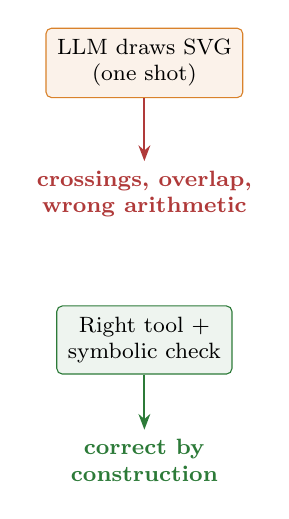
\begin{tikzpicture}[node distance=5mm]
      \node[llm] (a) {LLM draws SVG\\(one shot)};
      \node[below=8mm of a,text=kmred,align=center,font=\footnotesize] (b)
        {\textbf{crossings, overlap,}\\\textbf{wrong arithmetic}};
      \draw[ar,kmred] (a)--(b);
      \node[det,below=10mm of b] (c) {Right tool +\\symbolic check};
      \node[text=kmgreen,align=center,font=\footnotesize,below=7mm of c] (d)
        {\textbf{correct by}\\\textbf{construction}};
      \draw[ar,kmgreen] (c)--(d);
    \end{tikzpicture}
  \end{column}
  \end{columns}
\end{frame}

% ===================================================================
\begin{frame}{System at a glance}
  Three in-process components and a browser front-end.
  \vspace{2mm}
  \begin{center}
  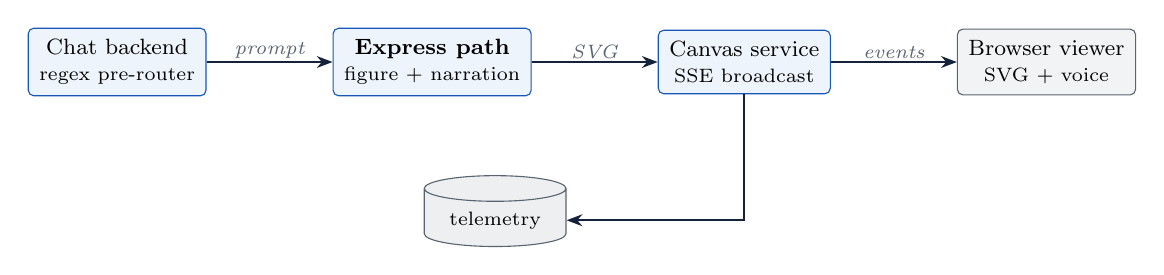
\begin{tikzpicture}[node distance=12mm and 16mm]
    \node[box] (chat) {Chat backend\\\scriptsize regex pre-router};
    \node[box,right=of chat] (exp) {\textbf{Express path}\\\scriptsize figure + narration};
    \node[box,right=of exp] (canvas) {Canvas service\\\scriptsize SSE broadcast};
    \node[box,right=of canvas,draw=kmgrey,fill=kmgrey!8] (view) {Browser viewer\\\scriptsize SVG + voice};
    \draw[ar] (chat)--node[lab,above]{prompt} (exp);
    \draw[ar] (exp)--node[lab,above]{SVG} (canvas);
    \draw[ar] (canvas)--node[lab,above]{events} (view);
    \node[store,below=10mm of exp,xshift=8mm] (db) {telemetry};
    \draw[ar] (canvas) |- (db);
  \end{tikzpicture}
  \end{center}
  \footnotesize
  A learner types or speaks $\to$ the express path returns an SVG, a
  narration and a title $\to$ the canvas service writes them to disk and
  streams them via Server-Sent Events $\to$ the viewer renders the SVG and
  plays the narration \emph{in lock-step} with element highlights.
\end{frame}

% ===================================================================
\begin{frame}{The end-to-end pipeline}
  \vspace{1mm}
  \begin{center}
  \resizebox{\textwidth}{!}{%
  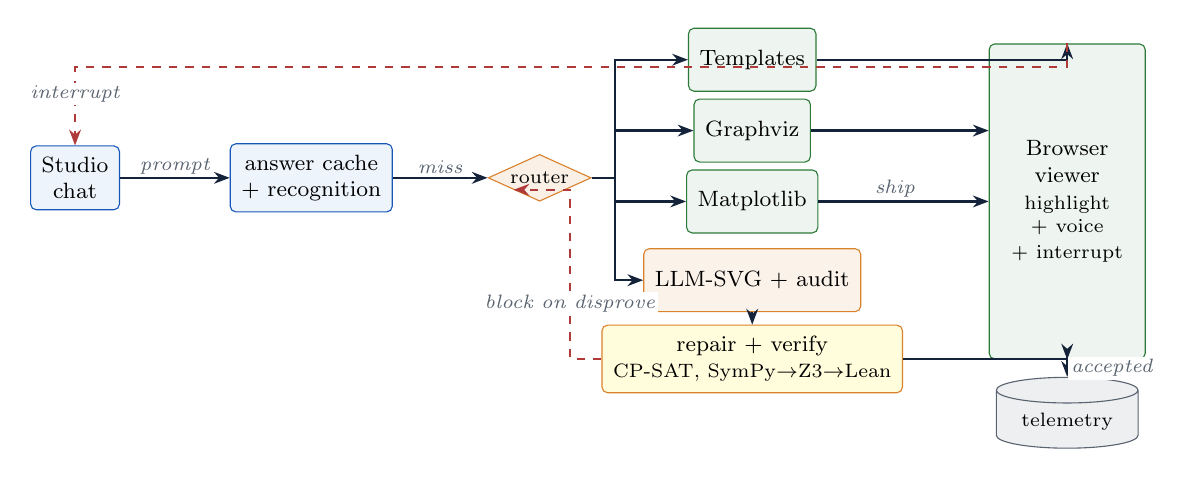
\begin{tikzpicture}[every node/.style={font=\footnotesize}]
    \node[box]  (chat)  at (0,3.7)  {Studio\\chat};
    \node[box]  (cache) at (3.0,3.7) {answer cache\\+ recognition};
    \node[dec]  (rt)    at (5.9,3.7) {router};
    \node[det]  (tmpl)  at (8.6,5.2) {Templates};
    \node[det]  (gv)    at (8.6,4.3) {Graphviz};
    \node[det]  (mpl)   at (8.6,3.4) {Matplotlib};
    \node[llm]  (llm)   at (8.6,2.4) {LLM-SVG + audit};
    \node[llm,fill=yellow!14,draw=kmorange] (rep) at (8.6,1.4)
         {repair + verify\\\scriptsize CP-SAT, SymPy$\to$Z3$\to$Lean};
    \node[box,fill=kmgreen!8,draw=kmgreen,minimum height=4.0cm,
          text width=1.7cm,align=center] (view) at (12.6,3.4)
         {Browser\\viewer\\[2pt]\scriptsize highlight\\$+$ voice\\$+$ interrupt};
    \node[store] (tel) at (12.6,0.6) {telemetry};
    \draw[ar] (chat)--node[lab,above]{prompt}(cache);
    \draw[ar] (cache)--node[lab,above]{miss}(rt);
    \draw[ar] (rt.east)-- ++(3mm,0) |- (tmpl.west);
    \draw[ar] (rt.east)-- ++(3mm,0) |- (gv.west);
    \draw[ar] (rt.east)-- ++(3mm,0) |- (mpl.west);
    \draw[ar] (rt.east)-- ++(3mm,0) |- (llm.west);
    \draw[ar] (tmpl.east) -| (view.north);
    \draw[ar] (gv.east) -- (gv.east-|view.west);
    \draw[ar] (mpl.east)-- node[lab,above,pos=.45]{ship}(mpl.east-|view.west);
    \draw[ar] (llm)--(rep);
    \draw[ar] (rep.east) -| (view.south);
    \draw[ar] (view)--node[lab,right]{accepted}(tel);
    \draw[arr] (rep.west) -- ++(-4mm,0) |- node[lab,below,pos=.2]{block on disprove}(rt.south west);
    \draw[arr] (view.north) |- ($(chat.north)+(0,1.0)$) -| node[lab,above,pos=.75]{interrupt}(chat.north);
  \end{tikzpicture}}
  \end{center}
  \vspace{1mm}
  \footnotesize
  Deterministic routes ship directly. The LLM-SVG path alone passes through
  layout repair and the symbolic verifier; a disproved claim is blocked.
\end{frame}

% ===================================================================
\begin{frame}{Stage 1 --- the express path}
  \begin{columns}[T]
  \begin{column}{0.6\textwidth}
  The single entry point \texttt{express\_figure(prompt)}:
  \begin{enumerate}\footnotesize
    \item detect language, classify the \emph{pedagogical archetype}
          (concept / worked example / \textbf{proof} / \dots),
    \item run the deterministic \textbf{routing cascade} (Stage 2),
    \item if nothing matches, the LLM emits SVG directly,
    \item \textbf{vision-audit retry loop}: rasterise with headless
          Chrome, ask GPT-4o to grade the pixels, re-emit up to 3 times,
    \item \textbf{symbolic verifier} (Stage 3) over the claims,
    \item \textbf{layout repair} (Stage 4) + narration binding.
  \end{enumerate}
  \end{column}
  \begin{column}{0.38\textwidth}
    \centering
    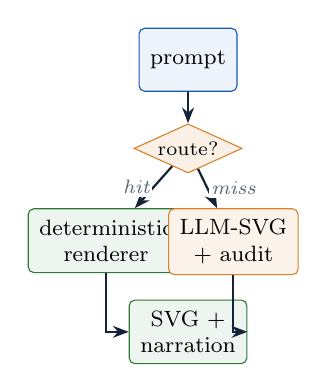
\begin{tikzpicture}[node distance=4mm]
      \node[box] (p) {prompt};
      \node[dec,below=of p] (r) {route?};
      \node[det,below left=6mm and -3mm of r] (d) {deterministic\\renderer};
      \node[llm,below right=6mm and -6mm of r] (l) {LLM-SVG\\+ audit};
      \node[box,below=16mm of r,fill=kmgreen!8,draw=kmgreen] (o) {SVG +\\narration};
      \draw[ar](p)--(r);
      \draw[ar](r)-- node[lab,left]{hit}(d);
      \draw[ar](r)-- node[lab,right]{miss}(l);
      \draw[ar](d)|-(o);
      \draw[ar](l)|-(o);
    \end{tikzpicture}
  \end{column}
  \end{columns}
\end{frame}

% ===================================================================
\begin{frame}{Stage 2 --- the multi-tool routing layer}
  \begin{center}
  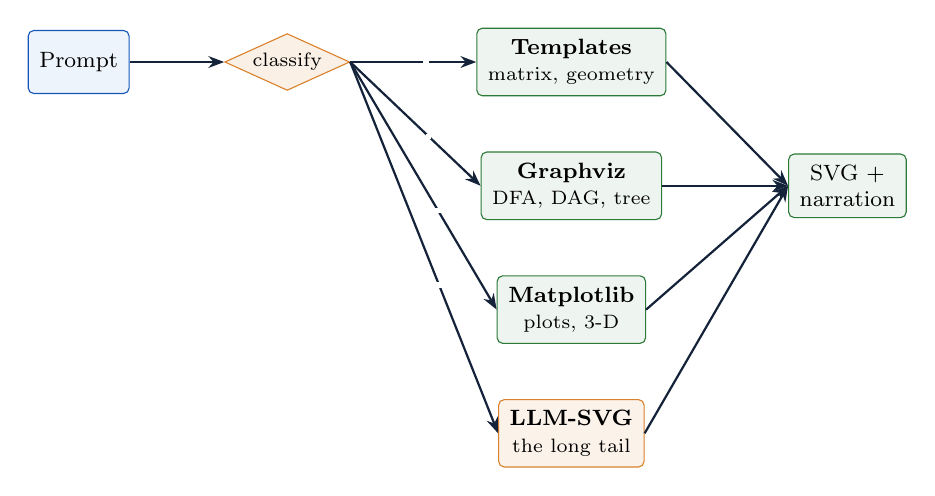
\begin{tikzpicture}[node distance=7mm and 12mm]
    \node[box] (p) {Prompt};
    \node[dec,right=of p] (c) {classify};
    \node[det,right=16mm of c] (t) {\textbf{Templates}\\\scriptsize matrix, geometry};
    \node[det,below=of t] (g) {\textbf{Graphviz}\\\scriptsize DFA, DAG, tree};
    \node[det,below=of g] (m) {\textbf{Matplotlib}\\\scriptsize plots, 3-D};
    \node[llm,below=of m] (s) {\textbf{LLM-SVG}\\\scriptsize the long tail};
    \node[box,right=16mm of g,fill=kmgreen!8,draw=kmgreen] (o) {SVG +\\narration};
    \draw[ar](p)--(c);
    \foreach \n/\lb in {t/matrix\textbar geom,g/graph,m/plot,s/fallback}
      {\draw[ar](c.east)-- node[lab,pos=.6]{}(\n.west);}
    \foreach \n in {t,g,m,s}{\draw[ar](\n.east)--(o.west);}
  \end{tikzpicture}
  \end{center}
  \footnotesize
  Each route is \textbf{correct by construction} for its family and
  sub-10\,s. Graphviz: zero edge crossings. Matplotlib: real 3-D
  projection, no canvas-filling blobs. Templates: every label computed in
  Python, never guessed. The LLM-SVG path absorbs everything else.
\end{frame}

% ===================================================================
\begin{frame}{Renderer-first: deterministic figures for fixed structures}
  When a whole \emph{class} of prompt has one fixed structure, we replace
  the LLM with a Python renderer that draws it correct-by-construction:
  \vspace{1mm}
  \begin{columns}[T]
  \begin{column}{0.5\textwidth}\footnotesize
    \textbf{Proofs \& reductions}
    \begin{itemize}\itemsep1pt
      \item ``$X$ is NP-complete'' (in-NP + reduction)
      \item Subset-Sum $\le_p$ Partition
      \item Infinitude of primes (Euclid)
      \item Fundamental Theorem of Calculus
    \end{itemize}
    \textbf{Probability \& stats}
    \begin{itemize}\itemsep1pt
      \item Bayes probability tree
      \item Normal distribution (68--95--99.7)
      \item Confusion matrix + precision/recall/F1
    \end{itemize}
  \end{column}
  \begin{column}{0.48\textwidth}\footnotesize
    \textbf{Fractals} (exact recursion)
    \begin{itemize}\itemsep1pt
      \item Mandelbrot \& Julia sets
      \item Barnsley fern (IFS)
      \item Koch, Sierpinski, Menger, Cantor
      \item Dragon curve, Pythagoras tree
    \end{itemize}
    \vspace{2mm}
    \begin{block}{\footnotesize Why it wins}
    \scriptsize Numbers are \emph{computed and asserted} in Python before
    drawing; proofs carry statement + steps + QED by construction. No
    hallucinated arithmetic, no failed proof rubric.
    \end{block}
  \end{column}
  \end{columns}
\end{frame}

% ===================================================================
\begin{frame}{Stage 3 --- multi-tier symbolic verifier}
  \begin{columns}[T]
  \begin{column}{0.52\textwidth}
  Math claims from the figure are checked on the \emph{synchronous}
  request path, cheapest tier first:
  \begin{itemize}\footnotesize
    \item \textbf{block} if a tier \emph{disproves} a claim,
    \item \textbf{defer} to the next tier if undecided,
    \item a disproved claim never reaches the learner.
  \end{itemize}
  \vspace{2mm}
  \footnotesize ``An editor with veto power over the slide deck'' --- not
  the model's own self-doubt.
  \end{column}
  \begin{column}{0.46\textwidth}
    \centering
    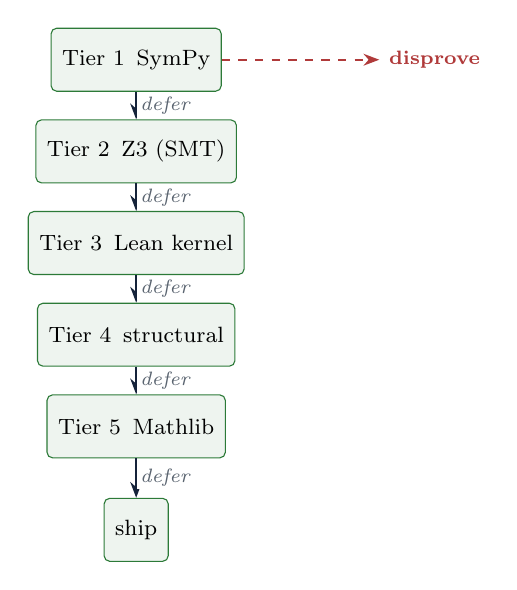
\begin{tikzpicture}[node distance=3.5mm]
      \node[det] (t1) {Tier 1 \,SymPy};
      \node[det,below=of t1] (t2) {Tier 2 \,Z3 (SMT)};
      \node[det,below=of t2] (t3) {Tier 3 \,Lean kernel};
      \node[det,below=of t3] (t4) {Tier 4 \,structural};
      \node[det,below=of t4] (t5) {Tier 5 \,Mathlib};
      \node[box,below=5mm of t5,fill=kmgreen!8,draw=kmgreen] (ok) {ship};
      \foreach \a/\b in {t1/t2,t2/t3,t3/t4,t4/t5,t5/ok}
        {\draw[ar](\a)-- node[lab,right]{defer}(\b);}
      \node[right=20mm of t1,kmred,font=\scriptsize\bfseries] (x) {disprove};
      \draw[arr] (t1.east) -- (x);
    \end{tikzpicture}
  \end{column}
  \end{columns}
\end{frame}

% ===================================================================
\begin{frame}{Stage 4 --- defensive layout repair}
  The LLM-SVG path alone passes through idempotent, deterministic repair
  passes before shipping:
  \vspace{1mm}
  \begin{center}
  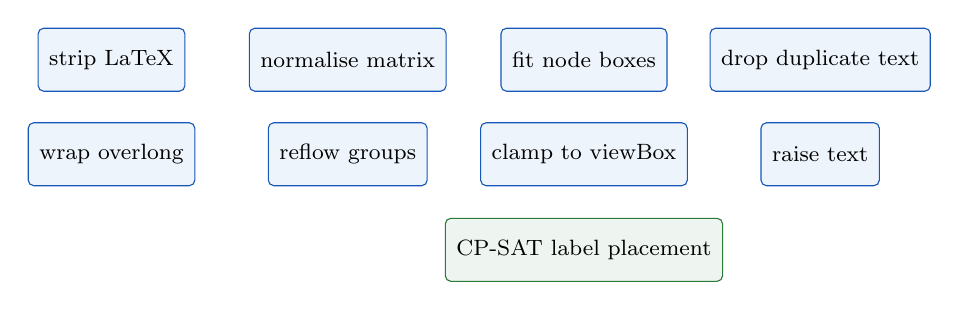
\begin{tikzpicture}[node distance=3mm and 5mm,every node/.style={font=\scriptsize}]
    \foreach \i/\t [count=\j] in
      {1/strip LaTeX,2/normalise matrix,3/fit node boxes,4/drop duplicate text,
       5/wrap overlong,6/reflow groups,7/clamp to viewBox,8/raise text}
      {\node[box] (n\j) at ({mod(\j-1,4)*30mm},{-floor((\j-1)/4)*12mm}) {\t};}
    \node[det,below=4mm of n7,fill=kmgreen!8,draw=kmgreen,minimum width=26mm] (cp)
      {CP-SAT label placement};
  \end{tikzpicture}
  \end{center}
  \vspace{1mm}
  \footnotesize
  Text-on-text collisions, out-of-bounds labels and duplicate captions are
  removed; \textbf{CP-SAT} (Google OR-Tools) then solves label placement to
  a global optimum --- the well-formed sub-problem a constraint solver
  already does better than any model.
\end{frame}

% ===================================================================
\begin{frame}{Stage 5 --- narration, voice and the live viewer}
  \begin{columns}[T]
  \begin{column}{0.55\textwidth}
  \begin{itemize}\footnotesize
    \item Narration is \textbf{phrase-timed}: each phrase highlights the
          exact element it describes.
    \item Timing is read from the WAV header, never estimated, so audio and
          highlights stay in lock-step.
    \item Voice: OpenAI \texttt{tts-1} (chosen over \texttt{tts-1-hd} for
          latency), with offline \textbf{Piper} as a no-cost fallback.
    \item \textbf{Narration interrupt}: the moment the learner types, hits
          send, or opens the mic, narration pauses.
    \item Multilingual: the prompt's language is detected and \emph{pinned}
          to every turn (no drift to another language).
  \end{itemize}
  \end{column}
  \begin{column}{0.43\textwidth}
    \centering
    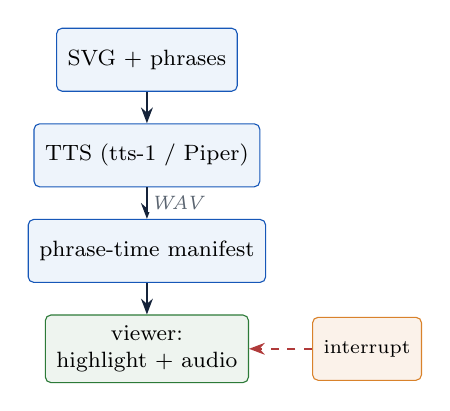
\begin{tikzpicture}[node distance=4mm]
      \node[box] (svg) {SVG + phrases};
      \node[box,below=of svg] (tts) {TTS (tts-1 / Piper)};
      \node[box,below=of tts] (man) {phrase-time manifest};
      \node[box,below=of man,fill=kmgreen!8,draw=kmgreen] (v) {viewer:\\highlight + audio};
      \draw[ar](svg)--(tts);\draw[ar](tts)--node[lab,right]{WAV}(man);
      \draw[ar](man)--(v);
      \node[llm,right=8mm of v,font=\scriptsize] (i) {interrupt};
      \draw[arr](i)--(v);
    \end{tikzpicture}
  \end{column}
  \end{columns}
\end{frame}

% ===================================================================
\begin{frame}{Consistency: taxonomy + answer cache}
  \begin{center}
  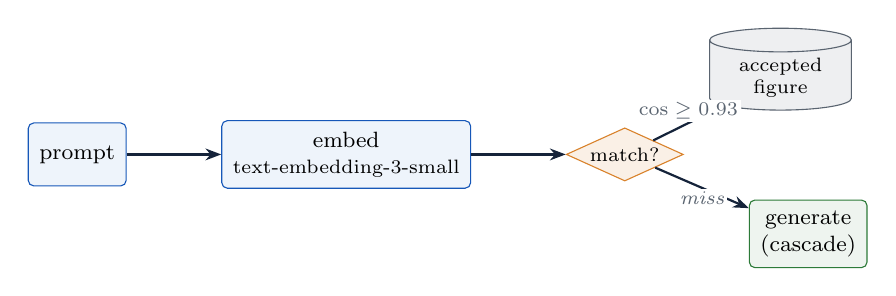
\begin{tikzpicture}[node distance=6mm and 12mm]
    \node[box] (p) {prompt};
    \node[box,right=of p] (emb) {embed\\\scriptsize text-embedding-3-small};
    \node[dec,right=of emb] (m) {match?};
    \node[store,above right=4mm and 12mm of m] (hit) {accepted\\figure};
    \node[box,below right=4mm and 12mm of m,draw=kmgreen,fill=kmgreen!8] (gen) {generate\\(cascade)};
    \draw[ar](p)--(emb);\draw[ar](emb)--(m);
    \draw[ar](m)-- node[lab,above]{$\cos\ge0.93$}(hit);
    \draw[ar](m)-- node[lab,below]{miss}(gen);
  \end{tikzpicture}
  \end{center}
  \footnotesize
  A near-verbatim repeat retrieves the prior accepted figure (consistency +
  cost). Threshold is high ($0.93$) on purpose: a precision sweep showed
  \emph{surface-similar but distinct} questions reach $0.70$--$0.78$, so
  broad paraphrase retrieval would mis-serve. An offline, admin-gated
  \textbf{curation loop} grows the taxonomy and promotes hot classes to
  deterministic renderers.
\end{frame}

% ===================================================================
\begin{frame}{Stage 6 --- the 6-hourly quality probe}
  \begin{center}
  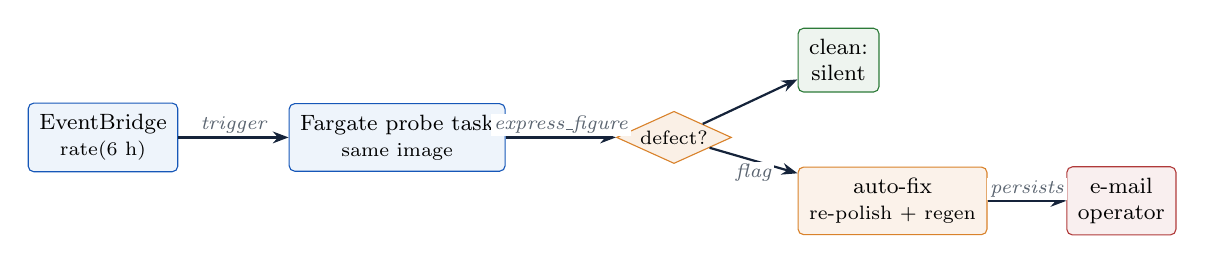
\begin{tikzpicture}[node distance=8mm and 14mm]
    \node[box] (sch) {EventBridge\\\scriptsize rate(6 h)};
    \node[box,right=of sch] (task) {Fargate probe task\\\scriptsize same image};
    \node[dec,right=of task] (insp) {defect?};
    \node[det,above right=4mm and 12mm of insp,draw=kmgreen,fill=kmgreen!8] (ok) {clean:\\silent};
    \node[llm,below right=2mm and 12mm of insp] (fix) {auto-fix\\\scriptsize re-polish + regen};
    \node[box,right=10mm of fix,draw=kmred,fill=kmred!8] (mail) {e-mail\\operator};
    \draw[ar](sch)--node[lab,above]{trigger}(task);
    \draw[ar](task)--node[lab,above]{express\_figure}(insp);
    \draw[ar](insp)--(ok);
    \draw[ar](insp)--node[lab,below]{flag}(fix);
    \draw[ar](fix)--node[lab,above]{persists}(mail);
  \end{tikzpicture}
  \end{center}
  \footnotesize
  Runs one demanding prompt through the \emph{real} production path every 6
  hours; structural checks catch overlap, out-of-bounds text, oversized
  elements, leaked internals. Optional bounded auto-fix re-attempts the
  figure; the operator is e-mailed only on \textbf{persistent} defects.
  Off by default; hard-stops at end of Aug 2026.
\end{frame}

% ===================================================================
\begin{frame}{Deployment topology (AWS)}
  \begin{center}
  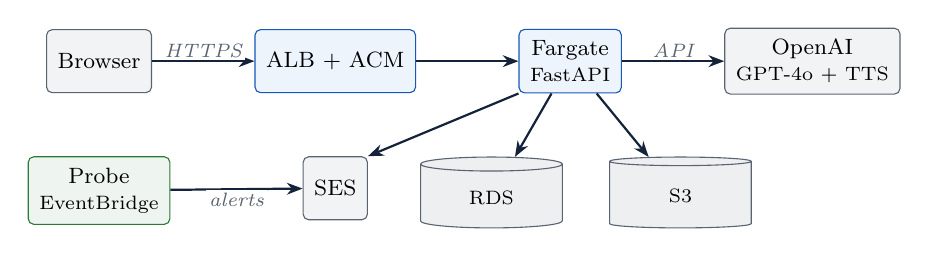
\begin{tikzpicture}[node distance=8mm and 13mm]
    \node[box,draw=kmgrey,fill=kmgrey!8] (u) {Browser};
    \node[box,right=of u] (alb) {ALB + ACM};
    \node[box,right=of alb] (far) {Fargate\\\scriptsize FastAPI};
    \node[box,draw=kmgrey,fill=kmgrey!8,right=of far] (oai) {OpenAI\\\scriptsize GPT-4o + TTS};
    \node[store,below=of far,xshift=-10mm] (rds) {RDS};
    \node[store,below=of far,xshift=14mm] (s3) {S3};
    \node[box,draw=kmgrey,fill=kmgrey!8,below=of alb] (ses) {SES};
    \node[box,below=of u,draw=kmgreen,fill=kmgreen!8] (pr) {Probe\\\scriptsize EventBridge};
    \draw[ar](u)--node[lab,above]{HTTPS}(alb);
    \draw[ar](alb)--(far);
    \draw[ar](far)--node[lab,above]{API}(oai);
    \draw[ar](far)--(rds);\draw[ar](far)--(s3);
    \draw[ar](far.south west)--(ses.north east);
    \draw[ar](pr)--node[lab,below]{alerts}(ses);
  \end{tikzpicture}
  \end{center}
  \footnotesize
  CDK stack: VPC, ALB+ACM (TLS 1.3), ECS Fargate (2 tasks, magic-link
  auth), RDS Postgres (telemetry), three S3 buckets, SES, EventBridge
  Scheduler. Deterministic figure generation needs none of it --- the
  package runs locally with just an OpenAI key.
\end{frame}

% ===================================================================
\begin{frame}{Closed loop: telemetry $\to$ fine-tuned open model}
  \begin{center}
  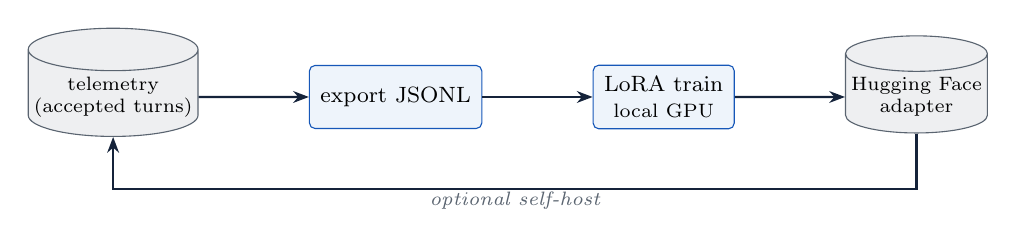
\begin{tikzpicture}[node distance=8mm and 14mm]
    \node[store] (db) {telemetry\\(accepted turns)};
    \node[box,right=of db] (exp) {export JSONL};
    \node[box,right=of exp] (gpu) {LoRA train\\\scriptsize local GPU};
    \node[store,right=of gpu] (hf) {Hugging Face\\\scriptsize adapter};
    \draw[ar](db)--(exp);\draw[ar](exp)--(gpu);\draw[ar](gpu)--(hf);
    \draw[ar](hf.south)-- ++(0,-7mm) -| node[lab,below,pos=.25]{optional self-host} (db.south);
  \end{tikzpicture}
  \end{center}
  \footnotesize
  Every accepted figure is a training example. A LoRA adapter on
  Qwen2.5-7B is distilled offline and published; the live service does not
  depend on it (a side artefact toward an offline-capable tutor).
\end{frame}

% ===================================================================
\begin{frame}{Tests}
  \begin{columns}[T]
  \begin{column}{0.5\textwidth}
  \textbf{516 pytest tests}, across $\sim$two dozen files:
  \begin{itemize}\footnotesize
    \item the 5-tier verifier chain,
    \item every deterministic template family,
    \item the new renderer-first routes (proofs, stats, \textbf{fractals}),
    \item the quality-probe inspection (transform-aware bounds, overlap),
    \item layout repair + CP-SAT schema,
    \item auth / sessions / rate-limit / content filter,
    \item telemetry, storage and export modes,
    \item Graphviz route, canvas API, narration-interrupt wiring.
  \end{itemize}
  \end{column}
  \begin{column}{0.48\textwidth}
    \begin{block}{Pre-deploy quality gate}
    \footnotesize A subset of prompts is run through the \emph{real}
    pipeline before every production deploy; a failing gate blocks the
    release. Flaky checks are retried (fail-both-to-block).
    \end{block}
    \begin{block}{Always-on monitoring}
    \footnotesize The 6-hourly probe (Stage 6) is the same idea applied to
    the \emph{live} service, continuously.
    \end{block}
  \end{column}
  \end{columns}
\end{frame}

% ===================================================================
\begin{frame}{Evaluation}
  \begin{columns}[T]
  \begin{column}{0.54\textwidth}
  \textbf{Blind multimodal judge} (GPT-4o vision scores figures from each
  model, neutral labels) on a diverse benchmark:
  \vspace{1mm}
  \begin{center}\footnotesize
  \begin{tabular}{lc}
  \hline
  Configuration & Total / 30 \\\hline
  GPT-4o (express path) & \textbf{22.9} \\
  Qwen2.5-7B base & 17.1 \\
  Qwen2.5-7B + LoRA & 13.8 \\\hline
  \end{tabular}
  \end{center}
  \end{column}
  \begin{column}{0.44\textwidth}
  \textbf{Lean-graded verifier sweep} at four-figure scale
  (difficulty 6/7/9/10): per-tier resolution measured; four systemic
  failure modes turned into permanent regression checks.
  \vspace{2mm}\par
  \textbf{Latency:} graph-shaped prompts drop from tens of seconds
  (LLM-SVG + retries) to \textbf{under 10\,s} (Graphviz).
  \vspace{2mm}\par
  \scriptsize\color{kmgrey} Numbers predate the latest renderer-first
  routes, which only move them favourably.
  \end{column}
  \end{columns}
\end{frame}

% ===================================================================
\begin{frame}{Takeaways}
  \begin{itemize}
    \item \textbf{Route, don't hope.} The right visual idiom comes from
          classifying the prompt, not from one LLM call.
    \item \textbf{Deterministic where structure is fixed.} Templates,
          proofs, stats and fractals are correct-by-construction --- and
          the arithmetic is \emph{asserted}, not guessed.
    \item \textbf{Symbolic verification on the hot path.} Block a disproved
          claim before it reaches the learner.
    \item \textbf{Mature tools beat new ML for layout.} Graphviz, matplotlib
          and CP-SAT have decades of layout engineering.
    \item \textbf{Watch production continuously.} A pre-deploy gate plus a
          6-hourly probe catch drift; fixes go in human-in-the-loop.
  \end{itemize}
  \vspace{3mm}
  \begin{center}\color{kmblue}\textbf{khayyammath.com}\quad\textbar\quad
  \color{kmgrey}\small github.com/khayyam-math \;\textbar\; DOI 10.5281/zenodo.20367146\end{center}
\end{frame}

\end{document}
